\chapter{State of the Art}\label{chap:sotart}

Since the emergence of \acrlong{AI}, \acrlong{ML} algorithms were used for medical data analysis. They provide helpful tools for analyzing datasets collected by modern hospitals equipped with monitoring and data collection devices \cite{kononenko_machine_2001}. Afterward, all that should be done is to use the stored data as an input to a program to run a learning algorithm. The derived result can further help the physicians diagnose the disease in the new patients by improving accuracy and diagnostic speed or conducting pertinent surveys. \

{\hskip 1em} \acrshort{ML} can also be combined with \acrfull{NLP} to determine the meaning of unstructured text data \cite{sidey-gibbons_machine_2019}. The use of respective techniques enable researchers to extract information from clinical incident reports \cite{ong_automated_2012}, social media activities \cite{greaves_use_2013}, and feedback about doctor performance \cite{gibbons_supervised_2017}. The generated information could be useful in early diagnosis. \

{\hskip 1em} \acrlong{ML} methods are well suited to predictions based on the given data. Combined with clinical data sources, they can generate prediction models for numerous clinical questions from sepsis early-warning systems to imaging diagnostics \cite{chen_machine_2017}. Even though almost none of these predictions can be held for a distant future (e.g., Will a patient have a heart attack within ten years?), they can provide sufficiently high accuracy predictions for short-term prognoses using the information of the current condition. Amid all the predictive algorithms in medicine, the only aspect that this work focuses on is mortality. \

\section{Mortality Prediction}

Patient death is a serious concern in hospitals, especially if it happens during treatment. A high hospital mortality ratio implies poor service provided which adversely affects the hospital reputation and negatively impacts the patient's family. Hence, it is of great interest to precisely predict the occurrence of in-hospital mortality to help the hospital to develop remedy plans and take precautionary measures, if feasible \cite{ma_gradient_2019}. \

{\hskip 1em} Various predictive models have been generated, and, as a general rule, they use different kinds of clinical data such as patient demographic information (age, gender, ethnicity, etc.) \cite{rau_prediction_2017}, medication information (surgery, equipment), measurement information (heart rate, blood pressure, temperature, etc.), disease information (disease history and current disease) \cite{sadeghi_early_2018}, and disease severity or medical notes \cite{jo_combining_2017, calvert_using_2016}. \

{\hskip 1em} There are also several medical scoring systems that predict the probability of patient mortality considering diverse parameters. \acrfull{APACHE} \cite{kho_interrater_2007}, \acrfull{SAPS} \cite{gall_new_1993}, and \acrfull{SOFA} are some examples of these systems. The mortality prediction is regarded as a binary classification problem in which patient death is labeled by “1,” and their survival until successfully discharge from hospital is labeled by "0" \cite{ma_gradient_2019}. \

{\hskip 1em} Dividing patients into two groups, "dead" or "alive," and identifying them correctly by the model is important since the ability to assign an expired patient to "dead" class (sensitivity), and the ability to assign a survived patient to "alive" class (specificity) shows how powerful the model is. This can be shown by \acrfull{AUC} in which both sensitivity and specificity should be as high as possible \cite{ma_gradient_2019}. \

\section{Glucose, Lactate and Mortality}

Some studies have been conducted about the association of glucose and lactate with the risk of death. Before referring to them, different levels of glucose and lactate must be presented. Sotello et al. \cite{sotello_glucose_nodate} defined glucose levels as in table~\ref{tab:glucoserange} and lactate levels, as in table~\ref{tab:lactaterange}, albeit there might be some slightly different categorizations of their levels in other articles. Note that the blood glucose/lactate level lower than normal is called hypoglycemia/hypolactatemia, and the blood glucose/lactate level higher than normal is called hyperglycemia/hyperlactatemia. \

\begin{table}[h]
\centering
\setlength\tabcolsep{50pt}
\caption{\label{tab:glucoserange}Blood glucose levels in both measurement units \cite{sotello_glucose_nodate}}
\begin{tabular}{@{}rcc@{}}
\toprule
\thead{}            & \thead{mg/dL}     & \thead{mmol/L}    \\ \midrule \midrule
\textbf{Low}        & \textless 60      & \textless 3.3     \\ \midrule
\textbf{Normal}     & 60-140            & 3.3-7.8           \\ \midrule
\textbf{High}       & 140-200           & 7.8-11.1          \\ \midrule
\textbf{Very High}  & \textgreater 200  & \textgreater 11.1 \\
\bottomrule
\end{tabular}
\end{table}

\begin{table}[h]
\centering
\setlength\tabcolsep{50pt}
\caption{\label{tab:lactaterange}Lactate levels in both measurement units \cite{sotello_glucose_nodate}}
\begin{tabular}{@{}rcc@{}}
\toprule
\thead{}            & \thead{mg/dL}     & \thead{mmol/L}    \\ \midrule \midrule
\textbf{Normal}     & \textless 36      & \textless 2.0     \\ \midrule
\textbf{High}       & 36-72.1           & 2.0-4.0           \\ \midrule
\textbf{Very High}  & \textgreater 72.1 & \textgreater 4.0  \\
\bottomrule
\end{tabular}
\end{table}

{\hskip 1em} Yi et al. \cite{yi_association_2017} and Zhou et al. \cite{zhou_fasting_2019} claimed that higher mortality is associated with low and high fasting glucose concentrations in the Korean and Chinese general population, respectively, according to their age and gender. Twito in \cite{twito_impact_2015} concluded that the elderly patient with \acrfull{DM} (aka diabetes), which is caused by elevated glucose level (hyperglycemia), has higher risks for mortality and morbidity in comparison with a non-diabetic person of the same age. \

{\hskip 1em} Smith et al. \cite{smith_base_2001} asserted that lactate and base excess could be used as outcome predictors for \acrlong{ICU} admitted patients so that patients with high mortality risk can be identified for further measures. Fifteen years later, Santi et al. \cite{santi_base_2015} replicated this study and realized that lactate and base excess are still useful disease severity indicators. In \cite{bakker_clinical_2013}, Bakker et al. expressed that hyperlactatemia usually reflects increased morbidity (organ failure) and high mortality. It means lactate monitoring is an important parameter for critically-ill patients to be early resuscitated. \

{\hskip 1em} Glucose and lactate are interrelated components of the carbohydrate metabolism; each can serve as a precursor for the other. Glycolysis is the sequence of metabolic reactions that convert glucose into pyruvate and then lactate, as an end product, with no oxygen requirement \cite{adeva-andany_comprehensive_2014}. This can be seen in figure \ref{fig:cellularlactate} from the cellular point of view. \

\begin{figure}[h]
\centering
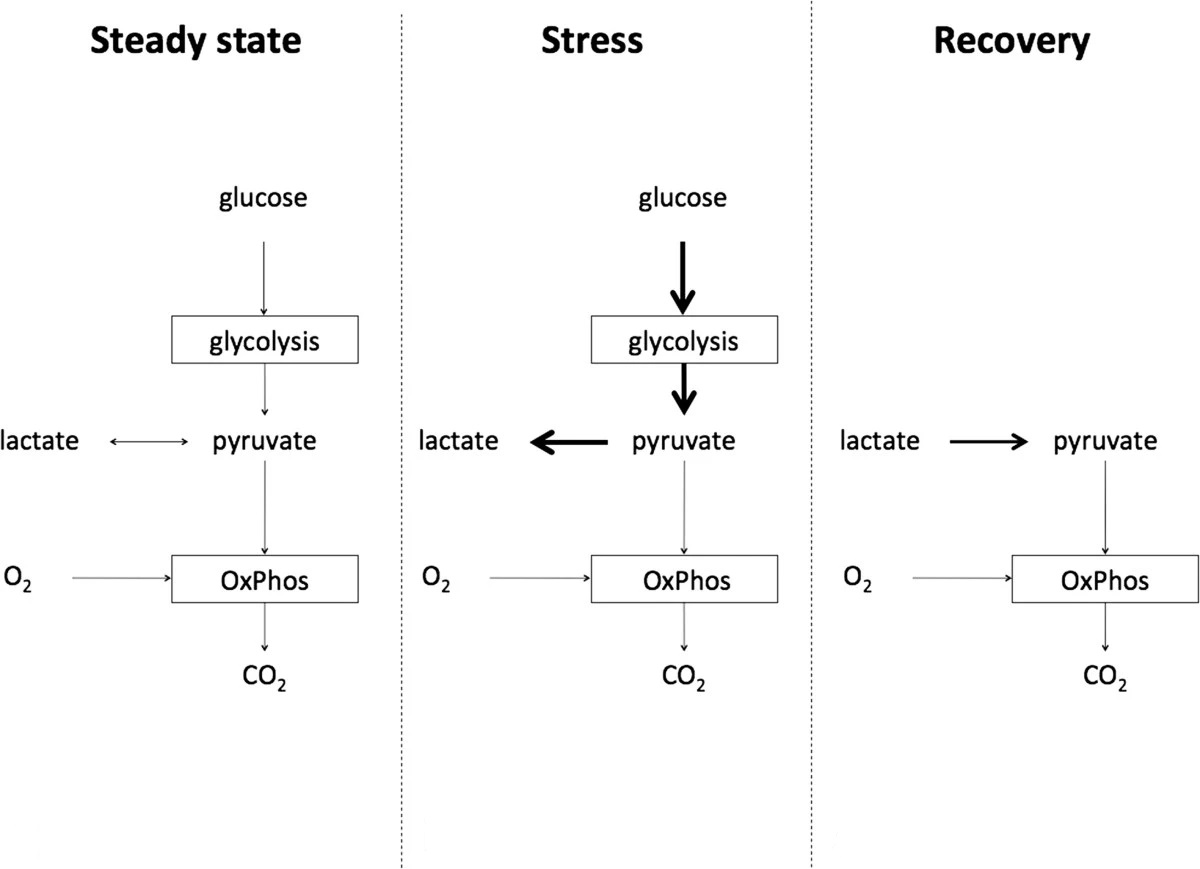
\includegraphics[width=14cm]{fig/chapter2/Cellular.jpg}
\caption{Lactate at the three different cellular levels \cite{bakker_clinical_2013}}
\label{fig:cellularlactate}
\end{figure}

{\hskip 1em} Figure \ref{fig:physiologicallactate} illustrates the association between glucose and lactate, physiologically. As it is shown, only the liver and the kidneys can reconvert lactate to pyruvate through the Cori cycle (denoted by \text{*}), which exports glucose and consumes \acrfull{ATP} (gluconeogenesis) \cite{kushimoto_lactate_2016}. This complex association of glucose and lactate brings about a hypothesis of taking both into account in identifying sicker patients. \

\begin{figure}[t]
\centering
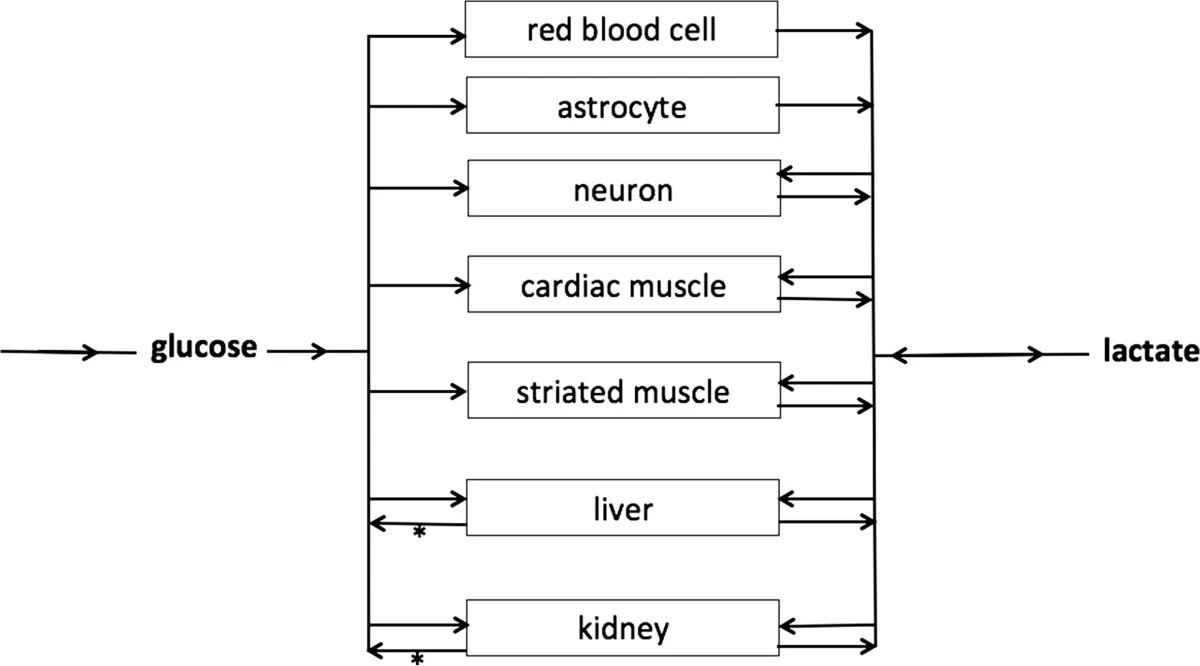
\includegraphics[width=14cm]{fig/chapter2/Physiological.jpg}
\caption{Lactate at the physiological level \cite{bakker_clinical_2013}}
\label{fig:physiologicallactate}
\end{figure}

{\hskip 1em} In \cite{sotello_glucose_nodate}, Sotello et al. argued that the glucose and lactate levels combination predicts mortality better than each value alone. Freire Jorge et al. claimed that hyperlactatemia combined with normal glucose levels is related to increased hospital mortality \cite{freire_jorge_association_2017}. Chen et al. stated that the lactate level, along with high- and low- glucose groups, is associated with in-hospital mortality. However, in the normal-glucose group, some medical scoring systems such as \acrshort{SOFA} or \acrshort{APACHE} should be utilized \cite{chen_impact_2019}. \

\section{eICU and Mortality}

The \acrlong{eICU-CRD} was published in 2019. Currently, more than 60 articles or book chapters have cited \acrshort{eICU} as their reference and are still counting ever since. Many of them focused on hospital mortality in critically ill patients. In \cite{byerly_vitamin_2020}, it is expressed that the combination of vitamin C and thiamine significantly reduces the mortality of critically ill septic patients. Deshmukh et al. \cite{deshmukh_explainable_2020} developed an \acrshort{ML} model that outperforms the \acrshort{APACHE} IVa scoring system in classifying the low-risk patients admitted with \acrfull{GI} bleed. The association of heart rate with hospital mortality in elderly and non-elderly critically ill patients was discussed in \cite{zhou_effect_2020}. Zhou et al. \cite{zhou_time_2020} studied the association of the proportion of time spent in oxygen saturation 95-99\% with reduced mortality in mechanically ventilated critically ill patients. They also surveyed the effect of age on the association of \acrfull{BMI} with in-hospital mortality \cite{zhou_obesity_2020}. Greco et al. \cite{greco_diabetes_2018} found that in non-diabetic patients, there is an association between glucose and lactate levels with glycemic variability, unlike in patients with \acrshort{DM}, where this relationship does not change by insulin remedy as the association is dramatically reduced. This study revealed that hyperlactatemia is associated with higher mortality and glucose levels along with \acrshort{DM} modifying this association in a three-way interaction.